% --*- coding:utf-8-unix mode:latex -*--
%\include{Begin}
%%%%%%%%%%%%%%%%%%%%%%%%%%%%%%%%%%%%%%%%%%%%%%%%%%%%%%%%%%%%%%%%%%%%%%%%%%%%%%%

\section{野外炊事}

\subsection{日時・場所}

\begin{tabular}{p{2zw}rp{38zw}}
  日時 & : & 2019年4月5日(金) 16:20 $\sim$ 19:00\\
  場所 & : & 野外炊事場
\end{tabular}

\subsection{目的}
新入生同士及び在学生,教職員が協力して料理を作ることにより,親睦や交流をはかるきっかけにしてもらう.

\subsection{タイムスケジュール}
% 時刻は必ず4桁(00:00)で書くこと!!!
\begin{longtable}{p{3zw}p{39zw}}
  16:20 & \textbf{◎ 野外炊事場到着}\\
        %& \ \  \textbullet \ \ \underline{野外炊事統括(高島)} \\
        %& \ \  - A棟で待機し,肉を渡す準備をする \\
        & \ \  \textbullet \ \ \underline{各班スタッフ} \\
        & \ \  - 各班のプラカードが置かれている机に誘導する \\
        & \ \  - 野外炊事場で点呼が完了したら小松に直接報告する \\
        & \ \  \underline{※雨天時:傘は邪魔にならない場所(机の下など)に置く} \\\\


  16:25 & \textbf{◎ 野外炊飯説明} \\
        & \ \  \textbullet \ \ 各班スタッフは席に着いたら説明があることを伝える \\
        & \ \  \textbullet \ \ 全員席に着いたら,小松は施設職員さんに説明をお願いする \\
        & \ \  \textbullet \ \ 施設職員さんより野外炊飯の説明が行われる \\
        & \ \  \textbullet \ \ 片付けの説明はよく聞いておく \\\\


        & \textbf{◎ アイスブレイキング} \\
        & \ \  \textbullet \ \ \underline{各班スタッフ} \\
        & \ \  - 班内の教職員,スタッフ,新入生で,自分の名前,呼んでほしいニックネーム,得意な料理,野外炊事の意気込みを言い合う(教職員のニックネームは割愛する) \\
        & \ \  - スタッフはこの意気込みから各自の力量を推測し,役割分担に役立てる \\
        & \ \  - 移動中に仲良くなったとスタッフが判断した場合は,アイスブレイキングを割愛してもよい \\\\

  16:30 & \textbf{◎ 調理開始(レシピ参照)} \\
        & \ \  \textbullet \ \ \underline{野外炊事統括(小松)} \\
        & \ \  - 班到着チェック後,本部にて食器・道具・食材の配布を行う(人数に注意) \\
        & \ \  - 全班チェック後は見回りをする \\\\

        & \ \  \textbullet \ \ \underline{各班スタッフ} \\
        & \ \  - 野外炊事の説明が終わったら,本部で食器・道具・食材を受け取る \\
        & \ \  - 班内で役割分担を行い,調理を開始する \\
        & \ \  - 各班のスタッフは新入生が全員映るように調理風景を撮る(スマホでも可) \\
        & \ \  - 薪係は薪置き場に薪を取りに行く \\
        & \ \  - 調理が完了した班から食事をとる(食事開始前に班ごとで集合写真を撮る) \\
        & \ \  - 食事が終わり次第片付けをする \\
        & \ \  - 怪我をした場合は,2班の所に連れて行き塩谷が対応し報告slackへ \\%(未変更)
        & \ \  - 各班,抜ける可能性がある人がいる班は2人構成,もしくは隣の班が2人構成になっているのでスタッフが抜ける場合には声をかけ,新入生だけの状態にしないようにする.\\
        & \ \  - 各班の代表は,男性教員方に野外炊事直後と22時以降のどちらでお風呂に入るか確認を取る \\
        & \ \  - 野外炊事直後に入浴を希望する男性教職員がいた場合は,報告slackに連絡する \\\\

  18:00 & \textbf{◎ 片付け開始}\\
        & \ \  \textbullet \ \ \underline{女性教員と先に入浴を希望する男性教員のいる班の代表} \\
        & \ \  - 食事が終了する頃に,班の代表は報告slackに連絡する \\\\

        & \ \  \textbullet \ \ \underline{渡辺,藤田} \\
        & \ \  - 女性教員と先に入浴希望の男性教員がいる全ての班(女性教員の班は6つ)から食事終了の連絡がきたら,それぞれの班の教職員に声をかけ,(就寝場所)に誘導する \\
        & \ \  - 渡辺が女性教員,藤田は報告slackを元に男性教員を誘導する \\
        & \ \  - 本館にて事務室でお願いし,第一・二研修室の鍵を開けてもらい,各自荷物を取り, 鍵を閉めてもらう \\\\

        & \ \  \textbullet \ \ \underline{鍵係(小谷)} \\
        % \ \  - 食事終了の連絡がきたら,事務室へ移動し,第一集会室・第二研修室・指導者棟(慎太郎と龍馬)・つどいの広間の鍵を受け取る \\
        %& \ \  - その後,第一集会室の鍵を開け待機する \\

        & \ \  - 小谷は報告slackを確認し,食事終了が早かった班が片付けが終わるタイミングを見る \\
        & \ \  - 一番最初に片付けが終わった班と一緒に本館に戻り,事務室でお願いして第一・二研修室を開けてもらう \\
        & \ \  - すべての荷物がなくなるまで見張りをする \\
        & \ \  - 教員紹介後見つかった忘れ物は,新入生が荷物を取りに来たとき,持ち主がいないか呼びかける \\\\

        & \ \  \textbullet \ \ \underline{野外炊事統括(小松)} \\
        & \ \  - 5班分の片付けが終了するころに職員の方を呼びに行く \\\\

        & \ \  \textbullet \ \ \underline{各班スタッフ} \\
        & \ \  - 各班スタッフは片付けが終わった時に報告slackに連絡する \\
        & \ \  - 片付けの仕方は幡多職員の指示に従う \\
        & \ \  - 食器の汚れをチェックする \\
        & \ \  - 大学の備品は一箇所に集めて机の上に置いておく \\\\


  18:45 & \textbf{◎ 片付けチェック}\\
        & \ \  \textbullet \ \ \underline{片付け:小松,立岩} \\
        & \ \  - 片付け終了後,各班の終了点呼を行う \\
        & \ \  - 全班完了次第,野外炊事統括(小松)は最終チェックをする.(ゴミの回収,忘れ物チェック) \\
        & \ \  - 用意した備品は全班終了後に小松が回収する \\
        & \ \  - ゴミはゴミ箱に捨てる \\\\

\newpage
        & \ \  \textbullet \ \ \underline{各班スタッフ} \\
        & \ \  - 片付けが終了し,職員のチェックを受けた班は,野外炊事統括(小松)に直接報告する \\
        %& \ \  - ?スタッフはコンテナを持ったまま班員を第一・二研修室に誘導し,各自荷物を取る \\
        %& \ \  - 入浴係(藤田,日下)は小谷から各指導者棟の鍵を受け取る \\
        %& \ \  - ?その後,コンテナを食堂で返却し,班員をくろしお棟へ誘導する(暗いので携帯のライトアプリを使用する) \\
        & \ \  - 19班(日下),小松の荷物を,1班(生野)は立岩の荷物を第一研修室で回収し宿泊部屋に向かう \\
        & \ \  - 就寝場所への誘導終了後,報告slackに連絡する \\\\

        & \ \  \textbullet \ \ \underline{鍵係(小谷)} \\
        & \ \  - 第一・二研修室に忘れ物がないか確認後,自分の荷物を持って就寝場所に移動する \\
        & \ \  - 第一・二研修室に物品があった場合は,第四研修室へ入れる \\
        & \ \  \underline{※雨天時:帰り道は十分に注意する} \\
        & \ \  \underline{※雨天時:傘を忘れない} \\\\

  19:00 & \textbf{◎ 終了(完全撤退)} \\\\
\end{longtable}

\subsection{人員配置}
\subsubsection{スタッフの役割}
\begin{itemize}
  \item 救急箱担当:塩谷
  \item 野外炊事統括:小松
  %\item ?車運転:西森
  \item 各班担当:各班2名〜3名
  %\item 肉担当:高島(三浦,下出が肉を持ってくるので,その肉を置き場所を確認する)
  \item 片付け:小松,立岩
  \item 鍵担当:小谷
  \item 女性教職員誘導:渡辺
  \item 男性教職員誘導:藤田
\end{itemize}

\subsubsection{班の割り当て}
\begin{itemize}
 \item 1班(生野,貞松),2班(塩谷,立岩),3班(伊崎,西森),4班(北村,小谷)
 \item 5班(丸田,小島),6班(吉田,藤田),7班(青山,堀川),8班(別役,高橋(慎))
 \item 9班(新田,宮尾),10班(高橋(龍),斎藤),11班(横田),12班(渡辺,小野)
 \item 13班(角原,以西),14班(高島,藤田(M2)),15班(石野),16班(江川)
 \item 17班(中島,野田),18班(小松,三浦),19班(東,日下),20班(新川,藤沢)
\end{itemize}

\newpage

\subsubsection{班内の役割(目安)}

準備時
\begin{itemize}
  \item 薪係:2名
  \item 食器係:2名
\end{itemize}

調理時
\begin{itemize}
  \item 火をおこす係:2名
  \item カレー係:2名
  \item 米を炊く係:1名
  %\item ?お茶を作る係:1名
  \item 皿を洗う係:1名
\end{itemize}

\subsubsection{野外炊事班}
\begin{figure}[H]
\begin{center}
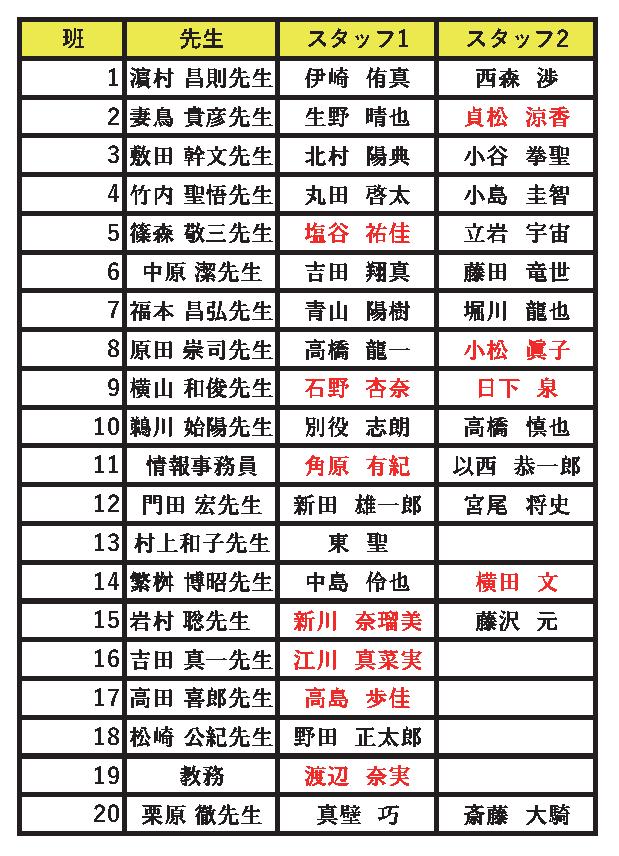
\includegraphics[scale=0.9]{./09/yagaisuijihanwake.eps}
\end{center}
\end{figure}

\newpage

\subsection{必要物品(1班分)}
\begin{itemize}
  \item ピーラー:1個(20個:幡青少年自然の家)
  \item 野外炊事班のプラカード:20個(名簿入り:誘導用)
  \item 野外炊事班用紙:20枚
  \item ゴミ袋:2班で1つ(11個:幡青少年自然の家)
  \item 軍手:20組(幡青少年自然の家)
  \item ふきん:1班に1つと予備4枚(24枚) 
  \item 新聞紙:20日分(幡青少年自然の家)
  \item うちわ(予備):10個(全体)
  \item チャッカマン:2個
  \item 着火剤:2個(全体)
  \item 食器用消毒液:1班1個と予備1個(21個)
  \item ライトアプリ(足下を照らすアプリであれば指定なし)
  \item 救急箱(大学からかりる)
  \item ポリ袋(予備用)20枚
  \end{itemize}

\subsection{全体配置(晴れ)}
\begin{figure}[h]
\begin{center}
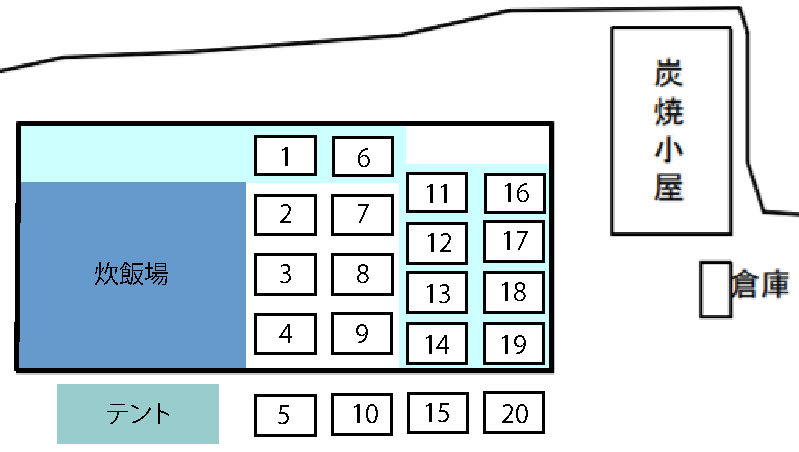
\includegraphics[width = 10cm]{./09/yagaisuiji.eps}
\label{fig:yagaihare}
\end{center}
\end{figure}

\newpage

\subsection{全体配置(雨)}
\begin{figure}[h]
\begin{center}
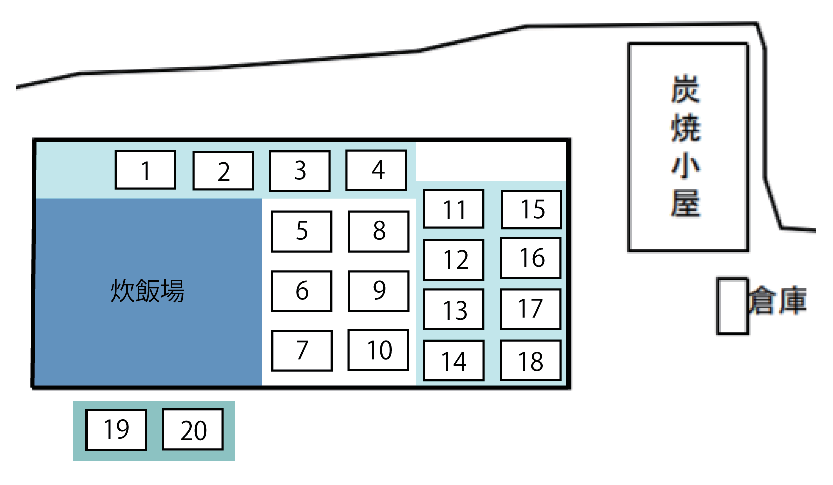
\includegraphics[width = 10cm]{./09/yagaisuijirain.eps}
\label{fig:yagaiame}
\end{center}
\end{figure}


\subsection{注意事項}
\begin{itemize}
  \item 新入生が手持ち無沙汰にならないように,人数分配を最初から終わりまで出来るだけ決めておく
  \item 時間の確認(終了時間のデッドラインや各作業の目安を確認する)
  \item 食器の個数と食材の確認
  \item 怪我に注意(火の扱い,包丁等)
  \item 食器を洗う際は,確実に汚れを落とす(点検をスムーズに行うため)
  \item 統括,各班スタッフ,新入生との「報連相」を密に行う
  %\item 鍵は担当が厳重に注意して管理する
\end{itemize}

\subsection{レシピ}
\begin{itembox}[l]{カレーのレシピ}
  \begin{enumerate}
    \item ピーラーでじゃがいも、にんじんの皮をむく
    \item 野菜は大きすぎると火が通らないので細かく薄く切る
    \item 肉は半分に切る
    \item お湯を沸かす(お茶用かつカレー非常時用に利用)
    \item 切った具材を鍋に入れ、ひたひたになるまで水を入れる(水を入れすぎない)
    \item 火にかける
    \item 沸騰まで放置する(フォーク等で刺し、じゃがいもやにんじんに穴があくかを確認する)
    \item ルーを開封前に細かく砕く
    \item 混ぜながらルーを入れる
    \item ルーが溶けたら終了
    \item カレーが濃いときはお茶用に沸かしているお湯で薄めると良い
  \end{enumerate}
\end{itembox}

\begin{itembox}[l]{ご飯のレシピ}
  \begin{enumerate}
    \item 米を研ぐ
    \item 米の表面から一差し指第2関節に行かないぐらいまで水を入れる
    \item 火にかける

    \item 最初は中火(底に火がふれるくらい)、途中で強火(はんごう全体が火に包まれるくらい)で加熱してやると美味しいご飯ができる
    \item 吹きこぼれて、吹きこぼれが乾いたら火から遠ざける(火にかけはじめて20分ほど待って吹きこぼれなかったらふたを開けて確認する)
    \item ご飯がべしゃべしゃの状態で炊けてしまったときはかまどの端っこの方(あまり火の当たらないところ)で1分ごとはんごうを回しながら水分を飛ばしてやると良い
  \end{enumerate}
※吹きこぼれている時には、絶対にふたは空けない
\end{itembox}

%\begin{itembox}[l]{お茶のレシピ}
%    \begin{enumerate}
%    \item やかんに水を入れて沸騰させる(カレーを薄めるためにお湯を使うかも知れないので早いうちからお茶っ葉を入れない)
%    \item 沸騰したらお茶っ葉をやかんに入れる
%    \item 10分ほど煮て火から遠ざける
%  \end{enumerate}
%※水を完全に沸騰させないと、味が不味くなる
%\end{itembox}

\subsection{備考}
\begin{itemize}
\item 基本的に各班代表者が報告slackへの連絡を行う
\item 火起こしの作業が遅れているときは他の班から人員を派遣する(火起こしが上手そうな人)
\item 進行状況は随時各班のスタッフが報告slackに連絡する(見回りにいけないとこもあるかも)
\item 宮尾は翌日の朝のつどいの旗揚げの新入生(3人)を野外炊事中にスカウトする(なるべく目立つ子を)
\end{itemize}


%%%%%%%%%%%%%%%%%%%%%%%%%%%%%%%%%%%%%%%%%%%%%%%%%%%%%%%%%%%%%%%%%%%%%%%%%%%%%%%
%\include{End}
